\سؤال{}

\begin{itemize}
	\item آ)
	همان‌طور که در کلاس درس و اسلایدها
	\footnote{اسلاید ۷، صفحه‌ی ۲۱.}
	 نیز اشاره شد، 
	\lr{SSE}
	معیار خوبی اندازه‌گیری خطا برای دسته‌بندی نیست؛ زیرا حتی برای داده‌هایی که درست دسته‌بندی شده‌اند اما فاصله‌ی زیادی با خط دارند، جریمه‌ی
	\footnote{\lr{penalty}}
	سنگینی برای آن‌ها نیز در نظر می‌گیرد و معیار نزدیکی به دسته‌بند 
	\footnote{\lr{classifier}}
	برای آن اهمیت دارد. در حالی‌که ممکن است دسته‌بندی داده‌ها به خوبی انجام گرفته باشد و خطای
	\lr{SSE}
	بزرگ باشد.
	
	\item ب)
	
	\begin{figure}[!hbpt]
		\centering
		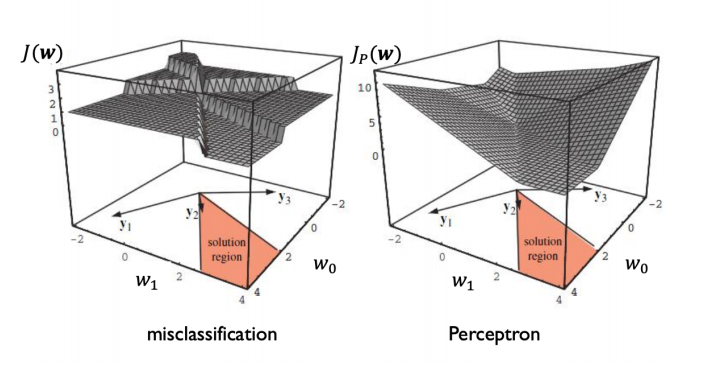
\includegraphics[scale=0.6]{./img/1b.png}
		\caption{مقایسه‌ی عمل‌کرد \lr{perceptron} و شمردن داده‌های \lr{misclassified}}
	\end{figure}
	با توجه به شکل،
	\footnote{ر.ک. اسلاید ۷، صفحه‌ی ۲۴.}
	 استفاده از روش 
	 \lr{perceptron criterion}
	 به ما این امکان را می‌دهد که به یک فضای محدب،
	 \footnote{\lr{convex}}
	 و پیوسته برسیم. به همین خاطر از روش‌های \lr{iterative} مانند \lr{gradient descent} برای رسیدن به جواب بهینه می‌توان استفاده کرد. این در حالی است که همان‌طور که مشاهده می‌شود، در روش شمردن تعداد داده‌های اشتباه دسته‌بندی‌شده، به شکلی می‌رسیم که مشتق
	 \footnote{\lr{gradient}}
	  آن، صفر است و نمی‌توان از روش‌های \lr{iterative} استفاده کرد. 
	  \item پ)
	  در حالت کلی سه روی‌کرد برای دسته‌بندی وجود دارد که دو نوع آن احتمالاتی و یکی نوع آن 
	  \lr{discriminant} است.
	  تابع خطای 
	  \lr{logistic regression}
	  از نوع احتمالاتی و 
	 \lr{perceptron}
	 از نوع 
	 \lr{discriminant}
	 است.
	  مزایای \lr{logistic regression}:
	  \begin{itemize}
	  	\item در مدل احتمالاتی، استنتاج
	  	\footnote{\lr{inference}}
	  	از تصمیم‌گیری 
	  	\footnote{\lr{decision}}
	  	جدا می‌شود.
	  	\footnote{در استنتاج به دنبال تخمین $p(t|x)$ هستیم اما در تصمیم‌گیری برای $x$ داده شده به دنبال $t$ بهینه هستیم.}
	  	\item از لحاظ محاسباتی کارا است.
	  	\item این امکان را به ما می‌دهد تا:
	  	\begin{itemize}
	  		\item ریسک را حتی اگر ماتریس وزن‌دهی خطا
	  		\footnote{\lr{loss matrix}} عوض شد، کمینه کنیم.
	  		\item \lr{Reject option} داشته باشیم.
	  		\item \lr{unbalanced class priors} داشته باشیم.
	  		\item مدل‌ها را ترکیب کنیم.
	  	\end{itemize}
	  \end{itemize}
  \item ت)
  به دلیل غیرخطی بودن تابع \lr{sigmoid}، برای 
  \lr{logistic regression}
  راه‌حل بسته‌ای
  \footnote{\lr{closed form solution}}
   وجود ندارد. 
   روش \lr{IRLS}
   	\footnote{\lr{Iterative Reweighted Logistic Regression}}
    می‌تواند سریع‌تر باشد. برای مثال اگر تابع $log-likelihood$ تقریبا درجه دو باشد، ممکن است فقط در چند مرحله به نقطه‌ی بهینه همگرا شود. به همین علت در کتاب 
    \lr{Bishop} نوشته شده است که:
  «اگر چه چنین روشی ممکن است منطقی به‌نظر برسد اما در حقیقت یک الگوریتم ضعیف است.»
 \footnote{\href{https://stats.stackexchange.com/questions/190298/choosing-irls-over-gradient-descent-in-logistic-regression}{سوال پرسیده شده در \lr{stackexchange}}}

 با توجه به دلایل مذکور، احتمال پیدا کردن ججاب بهینه، در روش \lr{IRLS} با تعداد عملیات کم‌تر، بیش‌تر است. 
 	\footnote{اسلاید ۷، صفحه‌ی ۶۰.}
	\item ث)
	\lr{Probit regression} نسبت به داده‌های پرت حساس‌تر است؛ زیرا اگر انتهای هر کدام از تابع‌ها را بررسی کنیم ، به نتیجه‌ی زیر می‌رسیم:
	$$
	\begin{cases}
		logistic \: regression \: tails  & \approx e^{-x} \\
		probit \: regression   & \approx  e^{-x^2}\\
\end{cases}
	$$
	به همین دلیل اگر داده‌ی پرتی به تابع \lr{probit regression} داده شود، وزن بیش‌تری به آن می‌دهد؛ بنابراین به داده‌های پرت نیز حساس‌تر است.
\end{itemize}